\documentclass[conference]{IEEEtran}
\IEEEoverridecommandlockouts
\usepackage{cite}
\usepackage{amsmath,amssymb,amsfonts}
\usepackage{algorithmic}
\usepackage{graphicx}
\usepackage{textcomp}
\usepackage{xcolor}
\usepackage{booktabs}
\usepackage{multirow}
\usepackage{url}
\newcommand{\TODO}[1]{\textcolor{red}{\textbf{#1}}}

\def\BibTeX{{\rm B\kern-.05em{\sc i\kern-.025em b}\kern-.08em
		T\kern-.1667em\lower.7ex\hbox{E}\kern-.125emX}}

\begin{document}
	
	\title{Deploying Lightweight Vision Models on the ESP32-S3: A Case Study in the ESP-DL Inference Pipeline}
	
	\author{
		\noindent\begin{minipage}[t]{0.47\textwidth}
			\centering
			{\sublargesize Youcef Harmouni}\\
			{\normalsize Institute of Electrical \& Electronic Engineering}\\
			{\normalsize (IGEE, ex.\ INELEC)}
		\end{minipage}%
		\hfill
		\begin{minipage}[t]{0.47\textwidth}
			\centering
			{\sublargesize Abdelaziz Bellili}\\
			{\normalsize Institute of Electrical \& Electronic Engineering}\\
			{\normalsize (IGEE, ex.\ INELEC)}
		\end{minipage}
		\\[8pt]
		\IEEEauthorblockN{Dr.\ Walid Touzout}
		\IEEEauthorblockA{Institute of Electrical \& Electronic Engineering\\(IGEE, ex.\ INELEC)}
	}
	
	\maketitle
	
	\begin{abstract}
		Deploying vision models on microcontrollers forces four design decisions that are usually
		studied separately: network width, whether to start from a pretrained backbone, whether to
		distill from a larger teacher, and how to quantize for integer-only inference. This case study
		evaluates them together in one pipeline (PyTorch training, ONNX export, ESP-PPQ INT8
		quantization to Espressif's \texttt{.espdl} format, and execution on an ESP32-S3 via ESP-DL),
		using a MobileNetV2-SSDLite detector on a six-class hand-gesture task. A width sweep from 46K
		to 547K parameters (single seed, no augmentation) gives the accuracy-capacity baseline.
		Pretraining raises F1 by 8.3 points at width 1.0 (546{,}774
		parameters). Distilling that model into an 86{,}870-parameter student raises F1 from 59.7\% to
		71.0\% (three-seed means), about two-fifths of the gap to the teacher. Quantization-aware
		fine-tuning (QAT) recovers about half of the post-training quantization (PTQ) loss at width 1.0
		(single seed); at width 0.3 the PTQ and QAT differences are within noise. On the device,
		inference latency tracks model size, not quantization scheme (94~ms at width 0.3, 469~ms at
		width 1.0), while fixed host-transfer overhead in our USB-Serial-JTAG harness takes about 51\%
		of the round trip for the small model and 17\% for the large one. Apart from the three-seed
		width-0.3 families, all results are single-seed runs on one task, and accuracy is scored by
		the host-side INT8 reference executor.
	\end{abstract}
	
	\begin{IEEEkeywords}
		TinyML, edge inference, microcontroller, ESP-DL, ESP32-S3, quantization, knowledge
		distillation, model compression
	\end{IEEEkeywords}
	
	\section{Introduction}
	
	Running a learned vision model on a microcontroller unit (MCU) is a fundamentally different
	engineering problem from running one on a phone or a server. An MCU-class device such as the
	ESP32-S3 has no operating-system-managed virtual memory, no dedicated GPU, and typically a few
	hundred kilobytes of on-chip SRAM (512~KB on the ESP32-S3, with optional external PSRAM~\cite{esp32s3ds}) alongside a flash budget measured in
	megabytes rather than gigabytes~\cite{david2021tflm,lin2020mcunet}. Floating-point throughput
	is limited relative to integer arithmetic, so practical deployments quantize both weights and
	activations to 8-bit integers and execute the entire forward pass without ever materializing a
	floating-point tensor~\cite{jacob2018quantization}. Every design decision upstream of
	deployment (how wide the network is, whether its weights started from a pretrained backbone,
	whether it was distilled from a larger model, and how quantization was applied) interacts
	with this budget, and the interactions are not always intuitive: a technique that clearly
	improves accuracy in an unconstrained setting can be worthless, or even actively
	counterproductive, once the model has to fit a fixed flash partition and answer within a fixed
	latency envelope on real silicon.
	
	Espressif's ESP-DL is a C/C++ inference library purpose-built for this constraint, targeting
	the ESP32, ESP32-S3, and ESP32-P4 chip families~\cite{espdlguide}. It defines its own compact model
	format, \texttt{.espdl}, and pairs with ESP-PPQ, a post-training quantization toolchain that
	converts a standard ONNX graph into an integer-only \texttt{.espdl} binary calibrated against a
	representative data sample. Unlike TensorFlow Lite Micro's interpreter-based
	approach~\cite{david2021tflm}, ESP-DL ships its own model format and quantization toolchain and
	exposes both post-training quantization (PTQ) and a quantization-aware training (QAT) path that
	fine-tunes the already-quantized graph directly, using ESP-PPQ's differentiable
	\texttt{TrainableGraph} representation rather than a separate simulated-quantization training
	run.
	
	This paper is a case study of what happens when four independent design levers (backbone
	width, ImageNet pretraining, knowledge distillation (KD), and the choice between PTQ and QAT)
	are exercised together inside this specific pipeline, on a single representative workload, and
	carried through to on-device latency measurements. We deliberately do not treat the detection
	architecture itself as a contribution: a single-scale MobileNetV2-SSDLite
	detector~\cite{sandler2018mobilenetv2,liu2016ssd} on a six-class hand-gesture recognition task,
	built from a sampled subset of the HaGRID dataset~\cite{kapitanov2024hagrid}, serves purely as a
	fixed, concrete workload against which the four levers can be compared on equal footing. The
	questions this study asks are practical ones an engineer actually faces when given an ESP32-S3
	and a vision task: how much does trimming network width cost in accuracy, and where does that
	cost stop being worth the parameter savings; how much of a pretrained model's advantage
	survives being distilled down to a deployable size; and whether the extra engineering effort of
	QAT is justified over plain PTQ at this scale, with accuracy scored by the host-side INT8 reference
	executor and latency measured on the chip.
	
	Our contributions are: (1) a parameter-count sweep from 46K to 547K parameters that
	quantifies the accuracy/capacity trade-off for a from-scratch, unaugmented, single-seed detector under this pipeline;
	(2) a measurement of ImageNet pretraining plus augmentation at fixed parameter count,
	controlling for architecture and data; (3) a knowledge-distillation experiment showing how
	much of a pretrained teacher's accuracy can be recovered inside a microcontroller-budget
	student; (4) a PTQ-versus-QAT comparison at width 1.0 and for the distillation student, including a
	calibration-set-size sensitivity study; and (5) real on-device latency and protocol-overhead
	measurements taken over the ESP32-S3's native USB-Serial-JTAG interface, characterizing how
	inference time and transfer overhead scale with model size independently of quantization
	scheme.
	
	\section{Related Work}
	
	\subsection{TinyML Inference Runtimes for Microcontrollers}
	
	TensorFlow Lite Micro (TFLM) established the now-standard pattern for MCU inference: an
	interpreter-based runtime that discards features common to full TensorFlow (dynamic memory
	allocation, virtual memory dependence, dynamic library loading) in exchange for portability
	across MCU targets with no operating system~\cite{david2021tflm}. CMSIS-NN provides optimized
	kernel implementations for Arm Cortex-M cores that TFLM and other runtimes can call into for
	common operators such as convolution and depthwise
	convolution~\cite{lai2018cmsisnn}. MCUNet takes a co-design approach one step further,
	jointly searching both the network architecture (TinyNAS) and the inference engine
	(TinyEngine) under a shared memory budget, and demonstrates that architecture and runtime
	choices made independently, the norm in most MCU deployments, leave measurable performance
	on the table relative to a jointly optimized pair~\cite{lin2020mcunet}. ESP-DL sits in the same
	family as an ESP32-specific runtime, but pairs with its own PTQ/QAT toolchain
	(ESP-PPQ) rather than delegating quantization to a separate front end~\cite{espdlguide}; this paper uses that
	toolchain's QAT-on-already-quantized-graph workflow and does not benchmark against TFLM. MLPerf Tiny offers a standard suite for comparing MCU systems on accuracy and latency~\cite{banbury2021mlperftiny}; we do not use it here.
	
	\subsection{Quantization for Edge Inference}
	
	Jacob \textit{et al.} formalized the integer-only inference scheme that underlies much of the current
	MCU quantization tooling: weights and activations are represented as 8-bit integers with one
	scale and zero-point per array (that is, per tensor), convolutions accumulate in 32-bit integer
	arithmetic, and a co-designed training procedure, which inserts simulated quantization into the
	computation graph during training, narrows the accuracy gap between the floating-point and
	integer models relative to naively rounding a fully-trained floating-point
	model~\cite{jacob2018quantization}. ESP-DL's ESP32-S3 target is narrower: it uses symmetric per-tensor quantization with power-of-two scales~\cite{espdldocs}. Post-training quantization (PTQ), which calibrates
	quantization scales from a small representative dataset without any further training, is
	computationally cheaper but generally incurs a larger accuracy cost than quantization-aware
	training (QAT), which fine-tunes the model with quantization effects simulated in the forward
	pass. At width 1.0 this paper's results follow that expected ordering, and we report the
	\emph{recovery ratio}, the share of the PTQ accuracy loss that QAT recovers; at width 0.3 the differences lie within evaluation noise and no ratio is claimed. For 8-bit weights and activations, PTQ is usually close to floating-point accuracy~\cite{nagel2021whitepaper}, so the 6.71-point PTQ loss at width 1.0 (Section~\ref{sec:ptqqat}) is larger than typical. ESP-DL's power-of-two constraint may contribute, but we did not test this.
	
	\subsection{Knowledge Distillation for Model Compression}
	
	Knowledge distillation, introduced by Hinton \textit{et al.}, trains a compact student network
	against a temperature-softened output distribution from a larger, already-trained teacher, on
	the premise that the relative confidences the teacher assigns to non-target classes carry
	information a hard-label cross-entropy loss discards~\cite{hinton2015distilling}. Applied to
	edge and embedded deployment specifically, results in the literature are mixed rather than
	uniformly positive: a recent MCU-class deployment study on animal re-identification, working
	under tight MCU memory limits, found that conventional feature-level distillation from a
	large teacher offered limited benefit over training a compact architecture directly once
	memory and input resolution were constrained as tightly as MCU deployment
	requires~\cite{chen2025animalreid}. In contrast, a concurrent study on vulnerable-road-user
	detection distilled a 43.7M-parameter YOLOv8-L
	teacher into an 11.2M-parameter YOLOv8-S student and found that the distilled student
	reached higher INT8 precision than a directly trained one, although the two students had nearly the same mAP and nearly the same INT8 degradation, and the large teacher collapsed under PTQ~\cite{karjol2026edgekd}. Our gain is in gesture-classification F1 rather than precision, and we observe no PTQ-cost advantage (Section~\ref{sec:kd}). Our setting is about two orders of magnitude smaller in parameters, and its deployment target is a microcontroller.
	
	\subsection{Backbone Design and Detection Head}
	
	MobileNetV2's inverted-residual, linear-bottleneck block is the standard building block for
	mobile- and edge-class vision backbones, and the same paper that introduces it also introduces
	SSDLite, a depthwise-separable variant of the SSD detection head designed to pair
	efficiently with it~\cite{sandler2018mobilenetv2}. SSD itself performs detection in a single
	forward pass by regressing offsets and class scores against a fixed set of anchor boxes tiled
	across one or more feature-map resolutions, avoiding the two-stage
	propose-then-classify pipeline of earlier detectors~\cite{liu2016ssd}. Neither is compared
	against alternative detectors; both serve as a fixed workload so that the architecture does
	not confound the four levers. For scale, full SSDLite-MobileNetV2 reports 22.1 mAP on COCO at 4.3M parameters~\cite{sandler2018mobilenetv2}; this is a smaller cut of that design (single tap, 128 pixels, six classes), so higher scores here mean an easier task, not a better detector.
	
	\section{Methodology and Hardware Deployment}
	
	\subsection{Detection Architecture and Task}
	\label{sec:data}
	
	\begin{table}[h]
		\caption{Detector geometry and anchor configuration.}
		\label{tab:geometry}
		\centering
		\begin{tabular}{ll}
			\toprule
			Parameter & Value \\
			\midrule
			Input resolution & $128 \times 128 \times 3$ \\
			Backbone output stride & 16 (feature map $8\times8$) \\
			Aspect ratios & $\{1.0,\ 1.8\}$ \\
			Anchors per cell & 2 \\
			Total anchors & $8 \times 8 \times 2 = 128$ \\
			Classes & 6 (fist, palm, like, ok, peace, point) \\
			\bottomrule
		\end{tabular}
	\end{table}
	
	The backbone is a MobileNetV2 truncated after its 14th feature block, giving an $8\times8$
	feature map at stride 16 from a $128\times128$ input. Two depthwise-separable heads,
	one for classification and one for localization, attach to this feature map and predict, per anchor
	location, class logits over six gesture classes plus an implicit background and four box
	regression offsets, following the standard SSD encoding with variances
	$(0.1, 0.1, 0.2, 0.2)$. Backbone capacity is controlled by MobileNetV2's \texttt{width\_mult}
	channel multiplier, which this study varies from 0.25 to 1.0 to trace the accuracy/parameter
	trade-off directly.
	
	Training and validation data are a sampled, pseudo-labeled subset of
	HaGRID~\cite{kapitanov2024hagrid}: six gesture classes (fist, palm, like, ok, peace, point)
	capped at 800 source images per class before bounding-box extraction, yielding 3{,}906 training
	and 433 validation images after the split. Ground-truth boxes are obtained via MediaPipe hand
	landmark detection~\cite{zhang2020mediapipe} over the raw HaGRID crops rather than from HaGRID's own annotations, since
	the sampled subset used here does not carry the original per-image bounding boxes; this is a
	practical labeling shortcut appropriate to a case study whose object of interest is the
	deployment pipeline rather than a state-of-the-art detector on this task. Label quality therefore caps measurable accuracy: the boxes track MediaPipe's hand estimate, and the learned component is chiefly the six-way gesture head.
	
	Every score in this paper comes from the single 433-image validation split. That split selects the best training checkpoint, supplies the PTQ calibration samples, selects the best QAT epoch, and scores the final models. No separate test set is held out, so absolute scores are mildly optimistic, and QAT scores include a best-of-10-epochs selection step. Each configuration is a single training run (seed 0), except the width-0.3 scratch baseline (augmented and unaugmented) and the KD student, which have three seeds each.
	
	The reported accuracy and macro-F1 are computed on the gesture label of the single highest-scoring detection above a 0.5 confidence threshold. A missed detection counts as an error (an extra wrong class: it lowers recall and accuracy but adds no precision term), so the deltas combine detection recall with gesture classification. Bounding-box localization is not scored. INT8 scores come from ESP-PPQ's reference executor on the host, which the ESP-DL documentation states can be aligned with board-side inference~\cite{espdldocs}. Only the latency measurements in Section~\ref{sec:latency} were taken on the device.
	
	\subsection{Training Regimes}
	
	Five model variants are trained under this pipeline, sharing the architecture in
	Table~\ref{tab:geometry} and the AdamW optimizer with cosine learning-rate annealing:
	
	\textbf{Scratch.} \texttt{width\_mult}$=0.3$, trained 120 epochs from random initialization on
	ground-truth labels only. This is the deployment-budget baseline: 86{,}870 parameters, chosen
	to sit inside a conservative $\sim$100K-parameter budget for ESP32-class deployment.
	
	\textbf{Pretrained.} \texttt{width\_mult}$=1.0$, backbone initialized from torchvision's
	ImageNet checkpoint (torchvision ships ImageNet weights for MobileNetV2 only at
	\texttt{width\_mult}$=1.0$, which fixes this variant's width) and fine-tuned 60 epochs on the
	gesture task. This variant is not itself deployment-budget-compliant; it exists to measure the
	accuracy ceiling pretraining offers and to serve as the distillation teacher.
	
	\textbf{Knowledge distillation.} A student at \texttt{width\_mult}$=0.3$ (identical
	architecture to the Scratch variant) is trained 120 epochs against a combined objective:
	
	\begin{equation}
		\mathcal{L} = \mathcal{L}_{\text{hard}} + \alpha\, \mathcal{L}_{\text{soft-cls}} +
		\beta\, \mathcal{L}_{\text{soft-loc}}
		\label{eq:kdloss}
	\end{equation}
	
	where $\mathcal{L}_{\text{hard}}$ is the standard SSD multi-box loss (hard-negative-mined
	cross-entropy plus Smooth-L1) against ground truth, $\mathcal{L}_{\text{soft-cls}}$ is the KL
	divergence between temperature-softened student and teacher class distributions
	($T=2.0$, following~\cite{hinton2015distilling}), and $\mathcal{L}_{\text{soft-loc}}$ is a
	Smooth-L1 term between student and teacher box regression outputs at the positive anchors the
	hard loss already selects. Both $\alpha$ and $\beta$ are set to $0.5$. The teacher is the
	Pretrained variant above, frozen and run in evaluation mode; only student parameters receive
	gradient updates. Reusing the Pretrained variant's own checkpoint as the teacher, rather than
	training a second nominally-identical model, removes any risk of the teacher's accuracy
	drifting from the number reported for the Pretrained variant itself.
	
	\textbf{Post-training quantization (PTQ).} Each trained model is exported to a static-shape
	ONNX graph (batch size 1, required by ESP-DL's target format) and quantized to INT8 via
	ESP-PPQ's \texttt{espdl\_quantize\_onnx}, calibrated against a subset of the validation split.
	
	\textbf{Quantization-aware training (QAT).} The PTQ-quantized graph is fine-tuned directly for
	10 epochs using ESP-PPQ's \texttt{TrainableGraph} representation and
	\texttt{forward\_with\_gradient}, at learning rate $1\times10^{-6}$ with momentum $0.937$.
	Because the batch-1 ONNX export bakes a fixed batch dimension into every reshape operation in
	the graph, the QAT loop processes one sample at a time and accumulates gradients over 64
	samples before each optimizer step, reproducing the effective batch size of the original
	training run without requiring the quantized graph to accept batched input. Ten QAT epochs
	against a 120-epoch main training budget is a deliberately small fraction ($\approx$8.3\% for the width-0.3 models, 16.7\% for the pretrained model) of
	total training cost, consistent with QAT's role here as a short
	fine-tuning pass on an already-converged model rather than a second full training run. The epoch with the highest validation F1 is retained, and the search starts from the PTQ score, so the retained model never scores below its PTQ starting point on the validation split.
	
	\subsection{ESP-DL Deployment Pipeline}
	
	\begin{figure}[h]
		\centering
		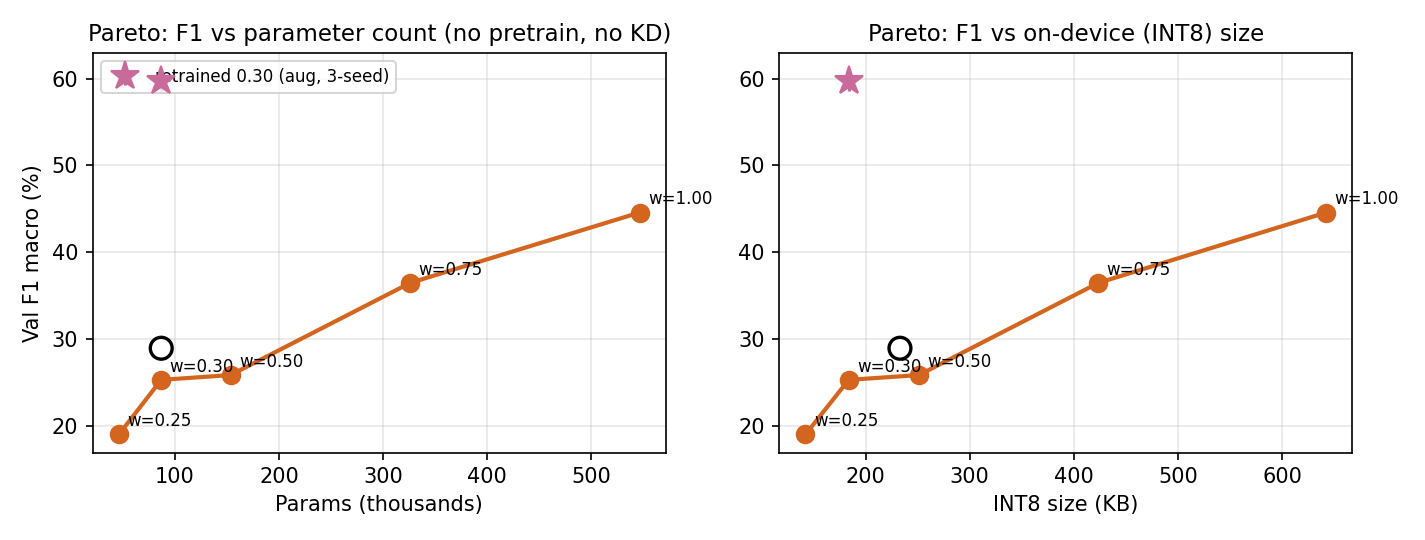
\includegraphics[width=\columnwidth]{figs/fig_scratch_width_pareto.png}
		\caption{Width sweep, from-scratch fp32 validation F1 versus parameters. Orange points are single-seed without augmentation; the line joins only the steps resolved by bootstrap CIs (0.50 to 1.00). The hollow point is the width-0.3 three-seed unaugmented mean (Table~\ref{tab:widthsweep} lists the overfit single-seed run instead). The pink star is the width-0.3 baseline with augmentation (three-seed mean $\pm$ SD), so its protocol differs from the sweep.}
		\label{fig:widthpareto}
	\end{figure}
	
	The quantized graph is exported to Espressif's \texttt{.espdl} binary format, a FlatBuffers-based
	container analogous to ONNX, and linked into an ESP-IDF firmware image as a binary blob referenced by linker symbol. The
	target hardware is an ESP32-S3 (dual-core Xtensa LX7, 8~MB octal PSRAM, 16~MB flash). Input
	images are pre-quantized on the host to INT8 using the exponent ESP-PPQ assigns the input
	tensor (an exponent of $-7$ was assigned for every variant in this study, corresponding to a
	quantization scale of $2^{7}=128$ applied to a $[0,1]$-normalized RGB image (rounded and clipped to the INT8 range) with no ImageNet
	mean/standard-deviation normalization), transferred to the device, and run through ESP-DL's
	static execution graph; on-device timing is measured with \texttt{esp\_timer} around the model
	\texttt{run()} call in isolation from image transfer.
	
	All host-device communication uses the ESP32-S3's native USB-Serial-JTAG peripheral, exposed
	to the host as a standard serial device and requiring no external UART bridge chip. A one-byte
	command triggers image transfer; the device echoes back a single line reporting the predicted
	class, confidence score, on-device inference time, and on-device receive time in microseconds,
	which the host parses to separate model compute time from transfer and protocol overhead in
	the measured round trip.
	
	\section{Results and Hardware Characterization}
	
	\subsection{Evaluation Noise and Seed Baselines}
	\label{sec:noise}
	
	All fp32 scores are recomputed from the saved best checkpoints. Because the 0.5 confidence threshold turns a near-threshold detection into a hit or a miss, re-scoring a checkpoint in a fresh process can move one image: the width-0.75 and width-1.0 scratch models differ from their training-time logs by 0.08 and 0.27 F1 points, and we report the recomputed values. This sets a noise floor of roughly one image (0.2 accuracy points) on every comparison. The pretrained PTQ re-export differs from the earlier export by about three images (0.58 F1 points), and Table~\ref{tab:pretrainedcomparison} reports the re-export. Where a difference is discussed, we also give a paired bootstrap 95\% confidence interval (10{,}000 resamples of the 433 images, the same resample for both models). These intervals capture evaluation-set sampling noise only (bootstrap SD 1.4 to 2.5 F1 points per model) and do not include training-seed variance.
	
	The width-0.3 baseline was trained with three seeds using box-aware train augmentation (flip, scale and color jitter; seeds change only init and batch order): 60.81, 58.52, 59.78 F1 (mean 59.70 $\pm$ 1.15; accuracy 46.50 $\pm$ 1.64). Here and below, $\pm$ is the sample SD over seeds, and ``fresh seeds'' means these three augmented scratch seeds. The same three seeds without augmentation score 32.70, 24.26, 29.91 (mean 28.96 $\pm$ 4.30), so augmentation alone is worth +30.7 points paired. The original KD student was one such augmented seed (69.78); two more under identical settings score 71.36 and 71.87, for a KD family mean of 71.00 $\pm$ 1.09. Scratch-1.0 was retrained once with augmentation (78.61 F1, best epoch 69). The single-seed width-0.3 run in Table~\ref{tab:widthsweep} (25.32, no augmentation) memorized its 3,906 training images (loss down to 0.02, validation stuck), so downstream comparisons use the three-seed means instead.
	
	\subsection{Width and Parameters}
	\label{sec:width}
	
	\begin{table}[h]
		\caption{From-scratch width sweep (no pretraining, no distillation), fp32. Single seed, no train augmentation; not repeated with augmentation or more seeds. $^\dagger$Overfit run (memorized the training set); excluded from step comparisons. Three-seed unaugmented mean 28.96 $\pm$ 4.30.}
		\label{tab:widthsweep}
		\centering
		\begin{tabular}{lrrr}
			\toprule
			width\_mult & Params & F1 macro (\%) & Accuracy (\%) \\
			\midrule
			0.25 & 46{,}182   & 19.04 & 12.70 \\
			0.30$^\dagger$ & 86{,}870   & 25.32 & 18.48 \\
			0.50 & 153{,}526  & 25.87 & 17.55 \\
			0.75 & 326{,}214  & 36.48 & 27.94 \\
			1.00 & 546{,}774  & 44.58 & 33.26 \\
			\bottomrule
		\end{tabular}
	\end{table}
	
	Table~\ref{tab:widthsweep} and Fig.~\ref{fig:widthpareto} sweep backbone width for single-seed models trained without augmentation. Validation F1 rises with width from 0.50 upward; paired bootstrap CIs (evaluation-set noise only) resolve the 0.50 to 0.75 step ($+10.61$ $[+4.4,+16.8]$) and the 0.75 to 1.00 step ($+8.10$ $[+2.0,+14.2]$). The overfit 0.30 row (25.32) is excluded from step comparisons, and no trend is claimed below width 0.50: the three-seed unaugmented 0.3 mean (28.96) lies above the single-seed 0.50 row (25.87). Width 0.75 (326{,}214 parameters) falls outside the $\sim$100K-parameter envelope this study targets for ESP32-class deployment. Width 0.3 is the deployment target, the widest inside the budget, at 59.70 $\pm$ 1.15 F1 over three augmented seeds. Even the largest width tested reaches only 44.58\% F1 from scratch without augmentation.
	
	\subsection{Pretraining Plus Augmentation at Fixed Parameter Count}
	
	\begin{table}[h]
		\caption{Pretraining plus augmentation at fixed parameter count (width\_mult$=1.0$, 546{,}774 params,
			identical data, fp32). Both rows single seed with augmentation; the comparison isolates pretraining.}
		\label{tab:pretrainisolation}
		\centering
		\begin{tabular}{lrr}
			\toprule
			Initialization & F1 macro (\%) & Accuracy (\%) \\
			\midrule
			Random (fresh seed, aug) & 78.61 & 69.05 \\
			ImageNet-pretrained, aug & 86.92 & 79.68 \\
			\midrule
			$\Delta$ & $+8.31$ pp & $+10.63$ pp \\
			\bottomrule
		\end{tabular}
	\end{table}
	
	The width-1.0 row of the from-scratch sweep (Table~\ref{tab:widthsweep}) and the Pretrained
	variant share architecture, parameter count, and training data. They differ in weight
	initialization, in epoch budget, and in augmentation: up to 120 augmented epochs from random initialization against 60 augmented fine-tuning epochs. The longer schedule favors the from-scratch model, and its validation F1
	peaked at epoch 69, so schedule alone does not explain the gap. Table~\ref{tab:pretrainisolation} therefore isolates pretraining's contribution. He \textit{et al.} report that ImageNet pretraining mainly speeds up convergence and that random initialization can catch up given enough iterations on COCO~\cite{he2019rethinking}; our 3{,}906-image training set is much smaller than COCO, so how far that result carries over here is untested. Pretraining adds +8.31 F1 points (+10.63 accuracy) at zero additional parameter cost, raising validation F1 from 78.61\% to 86.92\%: the smallest of the three training effects, which sharpens the central practical question the
	distillation experiment addresses: whether the teacher's remaining edge can be transferred to a model small
	enough to actually deploy, given that the pretrained checkpoint itself, at 546{,}774
	parameters and 2{,}283.5~KB in float32, is roughly 6.3$\times$ the parameters of the
	86{,}870-parameter deployment target.
	
	\begin{figure}[h]
		\centering
		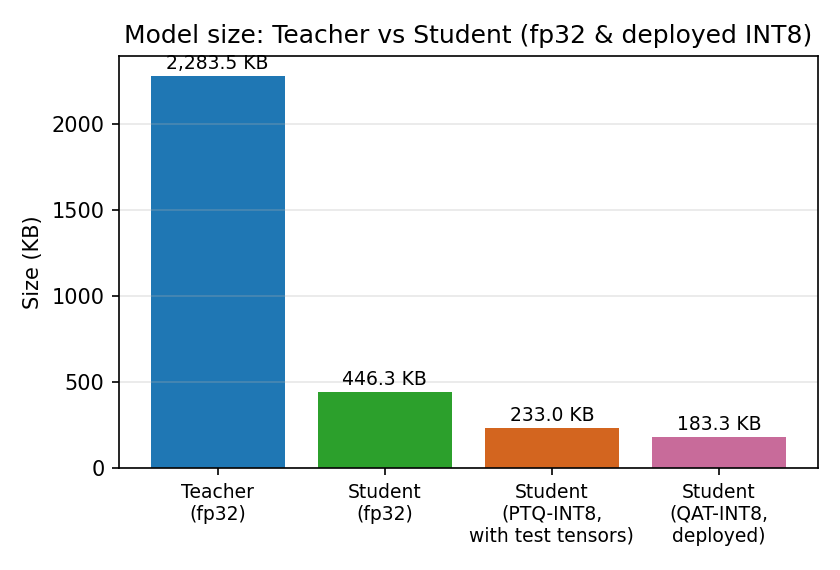
\includegraphics[width=\columnwidth]{figs/fig_kd_size_teacher_student.png}
		\caption{Exported model size: teacher float32 (width\_mult$=1.0$, pretrained) versus the distilled
			student (width\_mult$=0.3$) in float32, PTQ-INT8 with embedded test tensors, and deployed QAT-INT8.}
		\label{fig:kdsize}
	\end{figure}
	
	\subsection{Knowledge Distillation}
	\label{sec:kd}
	
	\begin{figure}[h]
		\centering
		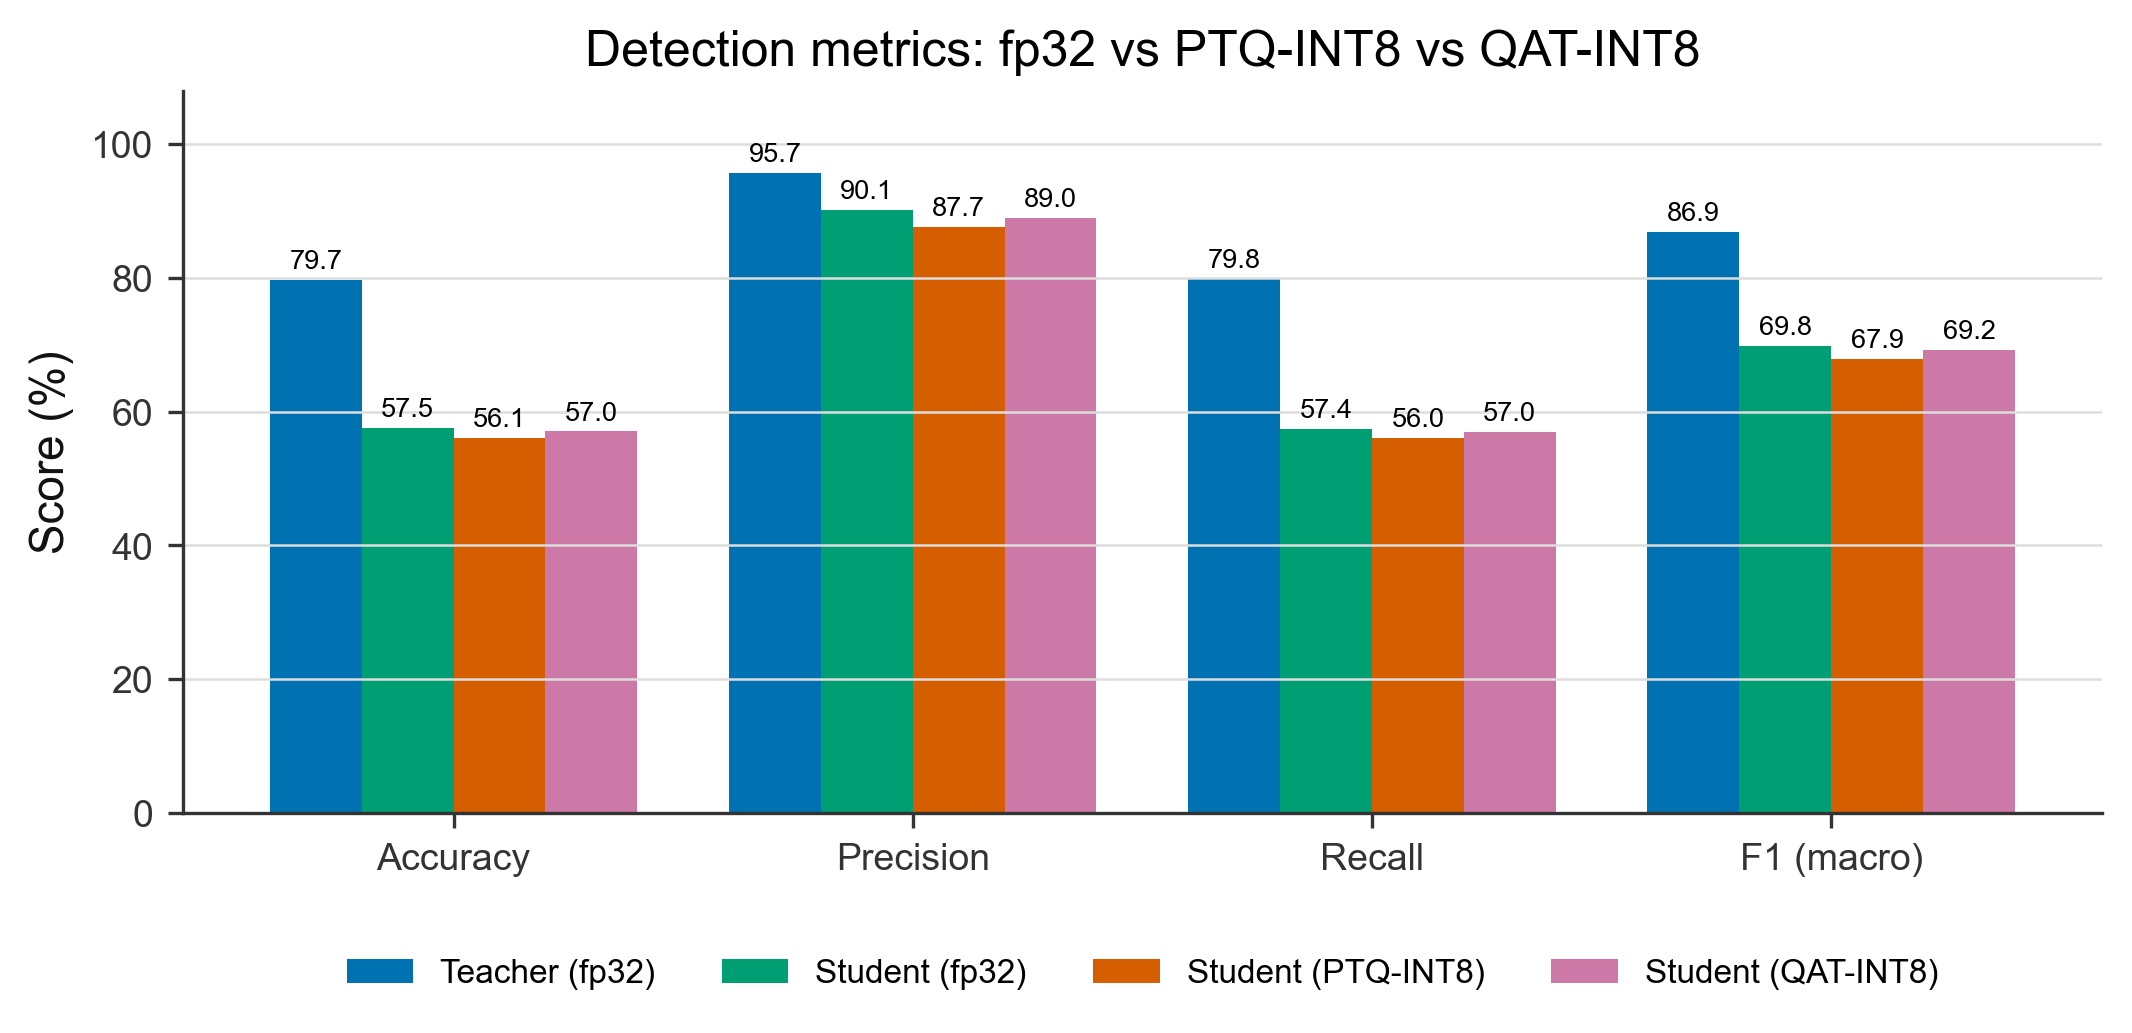
\includegraphics[width=\columnwidth]{figs/fig_kd_fp32_ptq_qat.png}
		\caption{Detection metrics for the knowledge-distillation student
			(width\_mult$=0.3$) across float32, PTQ-INT8, and QAT-INT8, alongside its float32 pretrained
			teacher (width\_mult$=1.0$) for reference. Bars show accuracy, precision, recall and macro-F1; student bars are the seed-0 student (family mean 71.00 F1).}
		\label{fig:kdcomparison}
	\end{figure}
	
	\begin{table}[h]
		\caption{Teacher/student/quantization comparison for the distillation pipeline. Student is
			width\_mult$=0.3$ (86{,}870 params); teacher is width\_mult$=1.0$, ImageNet-pretrained
			(546{,}774 params; teacher single seed). Student rows are the seed-0 student (family mean 71.00 F1). The PTQ file embeds ESP-PPQ test tensors ($\approx$49.7~KB); the QAT exports omit them. Integer weights occupy the same space in both.}
		\label{tab:kdcomparison}
		\centering
		\begin{tabular}{lrrr}
			\toprule
			Model & Size (KB) & F1 macro (\%) & Accuracy (\%) \\
			\midrule
			Teacher (fp32) & 2{,}283.50 & 86.92 & 79.68 \\
			Student (fp32) & 446.31 & 69.78 & 57.51 \\
			Student (PTQ-INT8) & 232.98 & 67.88 & 56.12 \\
			Student (QAT-INT8) & 183.31 & 69.20 & 57.04 \\
			\bottomrule
		\end{tabular}
	\end{table}
	
	Distillation lifts the width-0.3 student from 59.70\% (three-seed scratch mean) to 71.00\% (three-seed KD mean: 69.78, 71.36, 71.87 under the same teacher and settings) at fp32, an
	absolute gain of 11.30 points. That recovers about 42\% of the 27.22-point gap to its pretrained teacher (86.92\%, single seed, so teacher seed variance is not in the ratio), at the same 86{,}870 parameters. Our gain is large, unlike the limited benefit reported in~\cite{chen2025animalreid}. In~\cite{karjol2026edgekd}, KD left mAP unchanged but raised INT8 precision over direct training, at a much larger budget than here; the metrics differ, so the two results are not directly comparable. On PTQ cost this study observes no detectable KD advantage (one KD seed). Table~\ref{tab:kdcomparison}
	and Fig.~\ref{fig:kdcomparison} additionally show that PTQ costs the distilled student 1.90 F1
	points relative to its own fp32 result (69.78\% to 67.88\%), within the range of the three fresh scratch seeds (0.72--2.67; Section~\ref{sec:ptqqat}), though the KD student's PTQ cost is a single run.
	The QAT model reaches 69.20\% F1 (seed-0 student), within 0.58 points of the fp32 student (95\% CI of the QAT$-$fp32 difference $[-3.1,+1.9]$, so
	the two are indistinguishable on this validation set). The $\approx$49.7~KB size difference between the PTQ
	and QAT files traces to export settings (see the Table~\ref{tab:kdcomparison} caption and Fig.~\ref{fig:kdsize}).
	
	\begin{figure}[h]
		\centering
		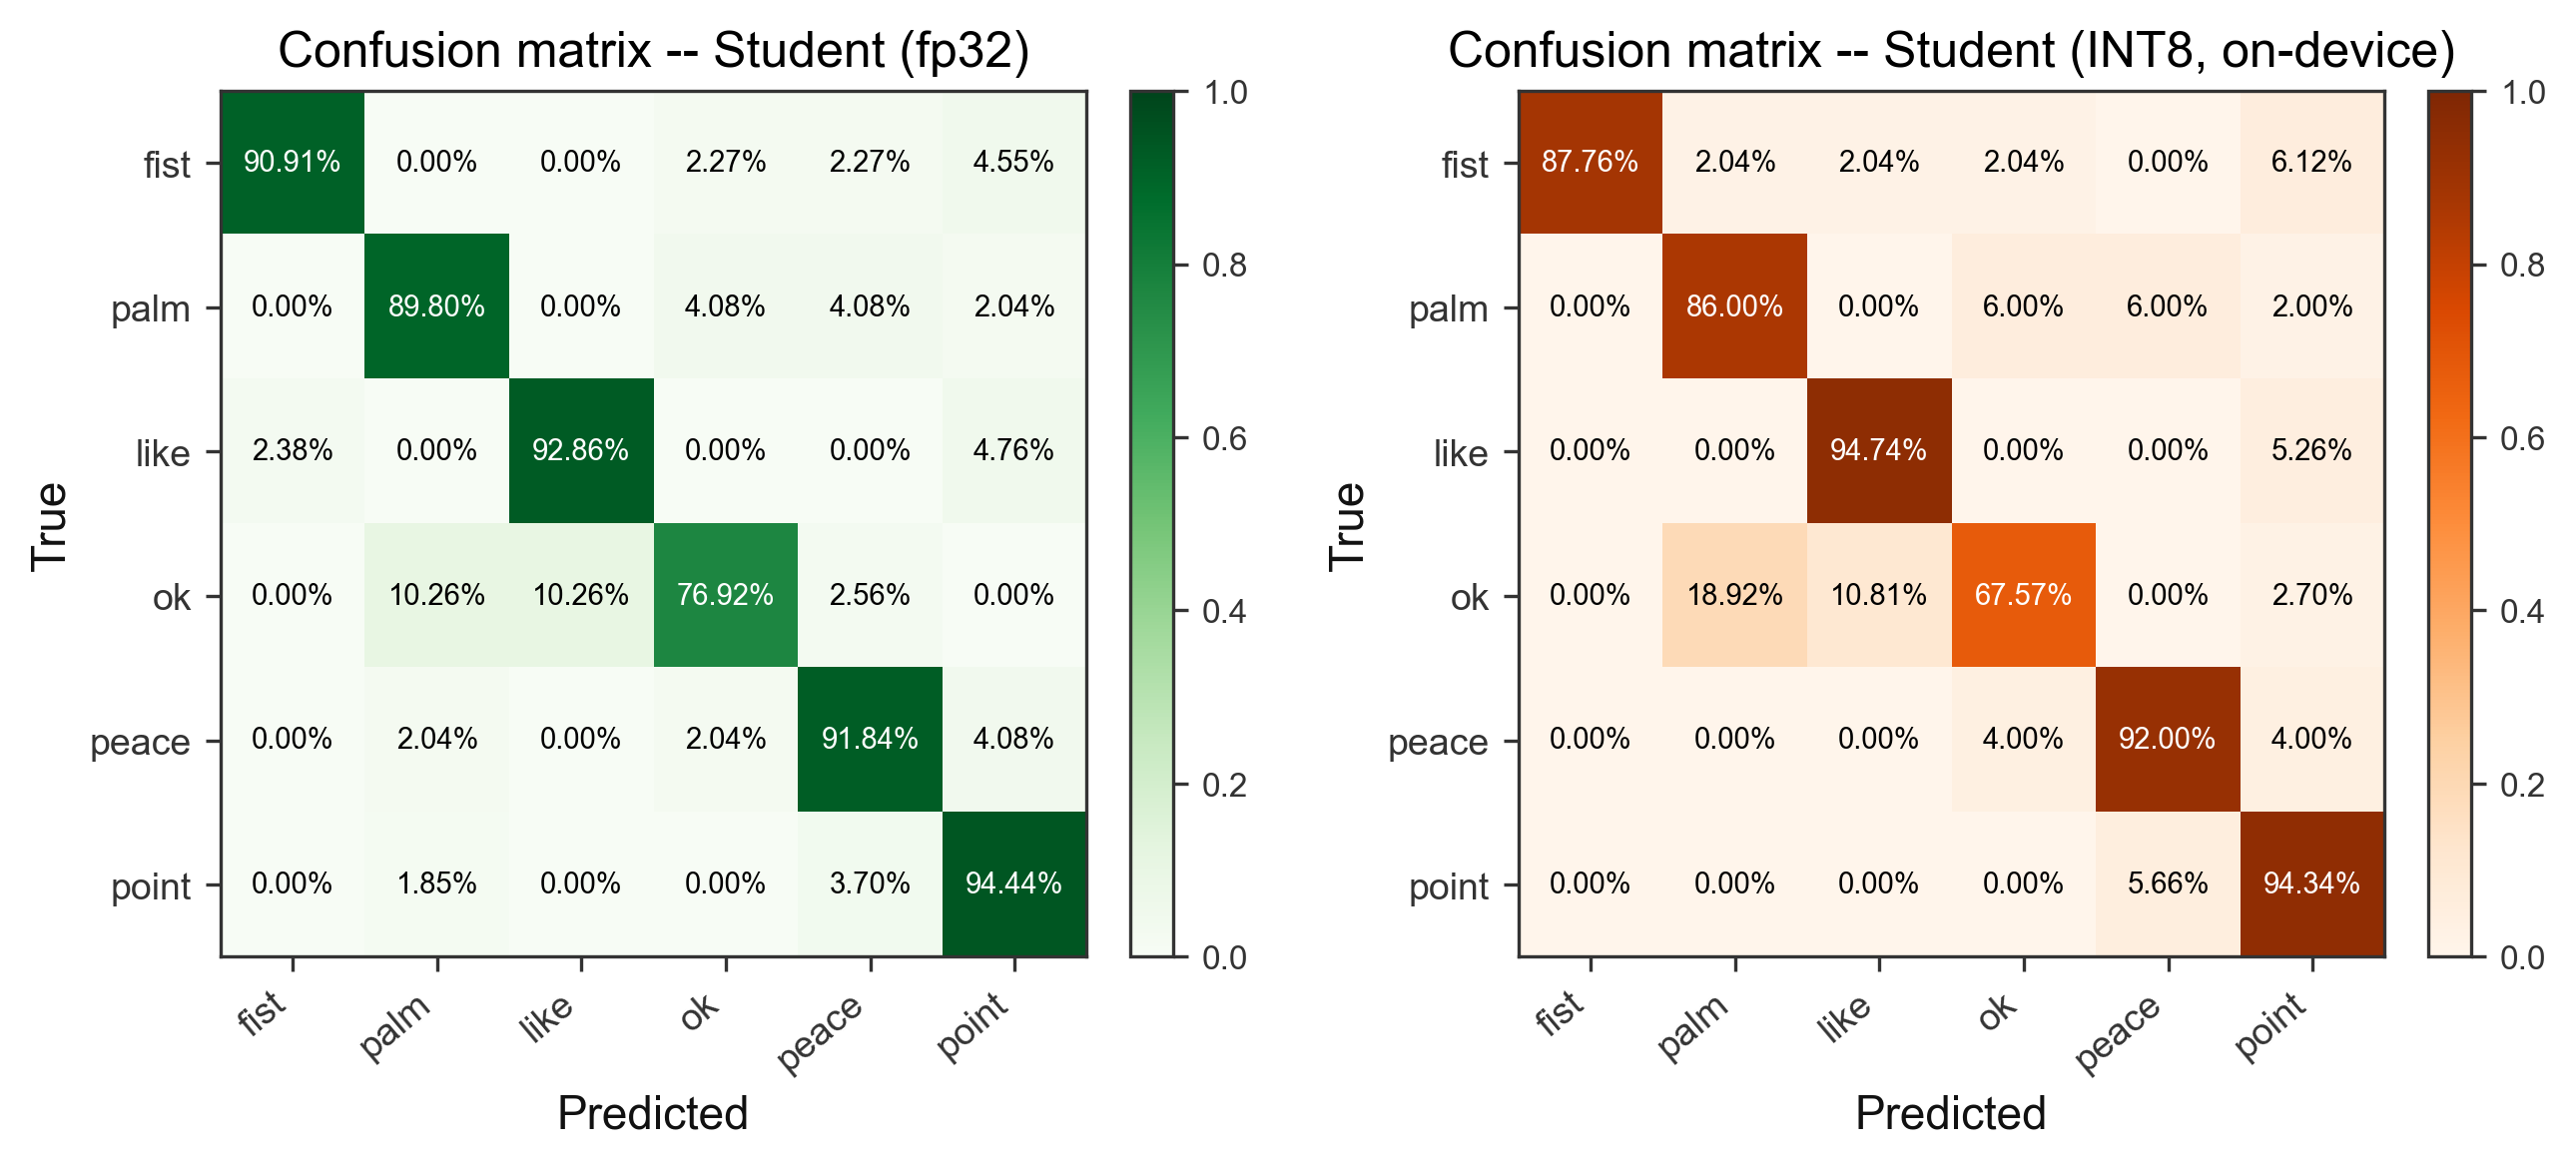
\includegraphics[width=\columnwidth]{figs/fig_confusion_student_qat.png}
		\caption{Per-class confusion matrices for the KD student: (a) fp32 (host-side) and (b) INT8 measured on-device. Cells are row-normalized \% per detected image of each true class.}
		\label{fig:confusion}
	\end{figure}
	
	Fig.~\ref{fig:confusion} shows per-class matrices for the fp32 student (a) and the on-device INT8 student (b), normalized over detected images; both runs detect 277 of 433. Errors concentrate in \emph{ok}: 76.92\% correct in fp32 (30/39, confused with \emph{palm} and \emph{like} at 10.26\% each) and 67.57\% in INT8 (25/37, confused with \emph{palm} in 18.92\% and \emph{like} in 10.81\%), while other classes score 86--95\% when detected. \emph{ok} and \emph{palm} share an open-hand silhouette at $128\times128$, which plausibly accounts for the asymmetry. Fig.~\ref{fig:demopred} shows example outputs.
	
	\subsection{PTQ, QAT, and the Calibration-Set Sensitivity}
	\label{sec:ptqqat}
	
	\begin{table}[h]
		\caption{Float32 / PTQ-INT8 / QAT-INT8 comparison for the pretrained (width\_mult$=1.0$)
			variant. Both INT8 files omit embedded test tensors; the PTQ row is the re-export scored in the final run.}
		\label{tab:pretrainedcomparison}
		\centering
		\begin{tabular}{lrrr}
			\toprule
			Model & Size (KB) & F1 macro (\%) & Accuracy (\%) \\
			\midrule
			Float32 & 2{,}283.50 & 86.92 & 79.68 \\
			PTQ-INT8 & 643.03 & 80.22 & 69.75 \\
			QAT-INT8 & 643.03 & 83.94 & 75.06 \\
			\bottomrule
		\end{tabular}
	\end{table}
	
	Table~\ref{tab:pretrainedcomparison} isolates the PTQ/QAT effect at width 1.0 (pretrained): PTQ costs 6.71 points
	(86.92\% to 80.22\%); QAT recovers 3.72 of those points (to 83.94\%), a recovery ratio of 55.5\% (single seed, best-of-10-epochs selected on the scoring split, so likely optimistic). The distilled width-0.3 student (Table~\ref{tab:kdcomparison}) loses only 1.90 points to PTQ (69.78\% to 67.88\%), within the fresh-seed range (0.72 to 2.67). Its QAT gain (1.32 points, Table~\ref{tab:kdcomparison}) is within evaluation noise, so no recovery ratio is claimed at width 0.3. Two readings fit the width-1.0 numbers. One is that the
	larger model has more capacity for QAT's short fine-tuning pass to still be exploring when
	training is cut off. The other is that the fixed 10-epoch budget stops the larger model earlier in its recovery. The study varies neither the QAT budget nor the seed, so it cannot separate these readings from each other or from
	run-to-run noise: the 55.5\% recovery is reported as an observation.
	
	\begin{figure}[h]
		\centering
		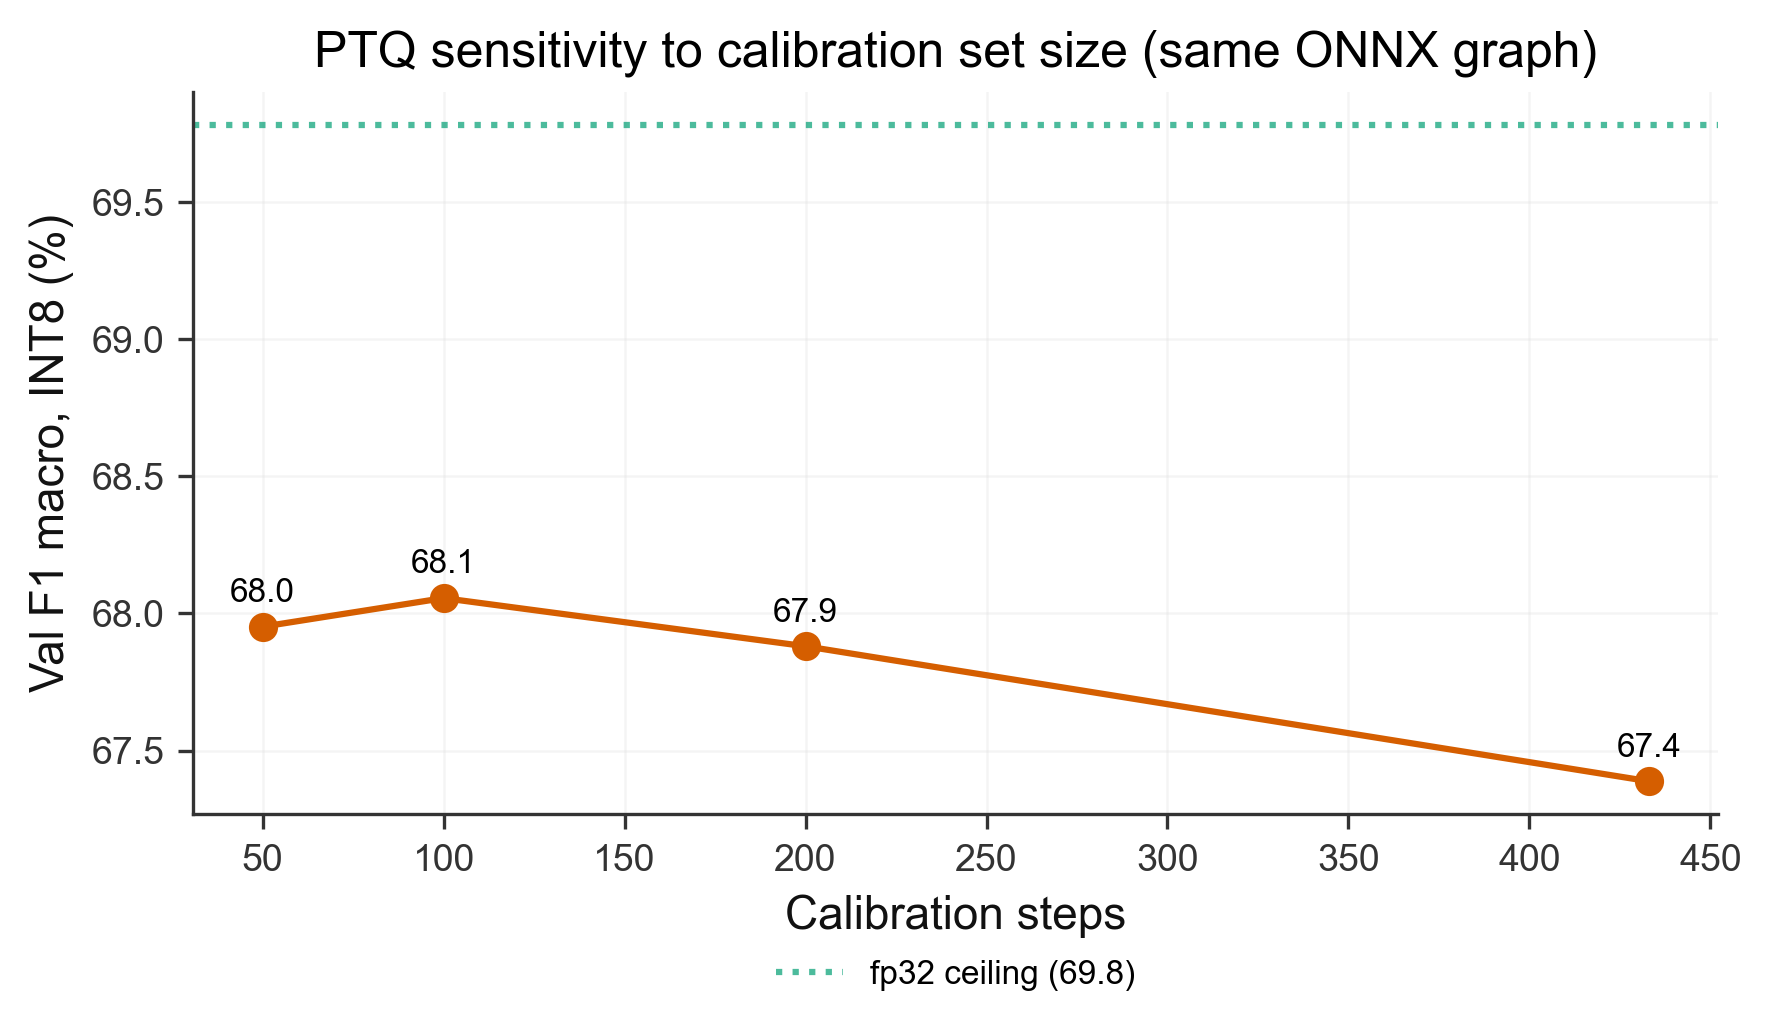
\includegraphics[width=\columnwidth]{figs/fig_calib_sensitivity.png}
		\caption{PTQ validation F1 (INT8, seed-0 distillation student) as a function of calibration set size,
			holding the underlying ONNX graph fixed. The fp32 ceiling is shown for reference; the y-axis is truncated.}
		\label{fig:calibsensitivity}
	\end{figure}
	
	\begin{table}[h]
		\caption{PTQ sensitivity to calibration set size, same ONNX graph (distillation student). The 200-step row is the main PTQ student of Table~\ref{tab:kdcomparison}; its file is larger because that export embeds test tensors.}
		\label{tab:calibsensitivity}
		\centering
		\begin{tabular}{lrrr}
			\toprule
			Calibration steps & Size (KB) & F1 macro (\%) & Accuracy (\%) \\
			\midrule
			50  & 183.98 & 67.95 & 56.35 \\
			100 & 183.98 & 68.06 & 55.89 \\
			200 & 232.98 & 67.88 & 56.12 \\
			433 (full validation set) & 183.98 & 67.39 & 54.97 \\
			\bottomrule
		\end{tabular}
	\end{table}
	
	Fig.~\ref{fig:calibsensitivity} and Table~\ref{tab:calibsensitivity} sweep the number of
	calibration samples ESP-PPQ uses to fit PTQ's quantization scales, holding the underlying ONNX
	graph fixed so that any change in accuracy is attributable to calibration data volume. Each
	row uses the first $N$ validation images in fixed order, a single draw per $N$. F1 varies by
	less than 0.7 percentage points across an 8.7$\times$ range in calibration set size (50 to
	433 samples), with the 100-step point highest and the full 433-sample pass lowest. On a
	433-image evaluation set a spread of that size cannot be separated from sampling noise, so the
	supported reading is that no benefit from larger calibration sets is detectable here. For this
	model and pipeline, a calibration sample of 50 to 100 images already matches the full-set
	result within that resolution. Across the three fresh seeds, PTQ exports with and without embedded test tensors differ by about 49.7 KB with identical scores (183.98/183.31/184.01 KB against $\sim$233.6 KB): the gap is packaging, stable across seeds. Fresh-seed PTQ costs are 2.67, 0.72, and 1.81 points (mean 57.97 $\pm$ 0.17 F1, PTQ cost 1.73 $\pm$ 0.98). Weight magnitudes agree between student and seeds: Fig.~\ref{fig:weightaudit} overlays absolute weight values for the KD student, the three fresh seeds, and the teacher. Student and seeds overlap compactly (means within 0.003, p99 within 0.01) with no heavy tails; the teacher's weights are smaller and concentrate near zero.
	
	\begin{figure}[h]
		\centering
		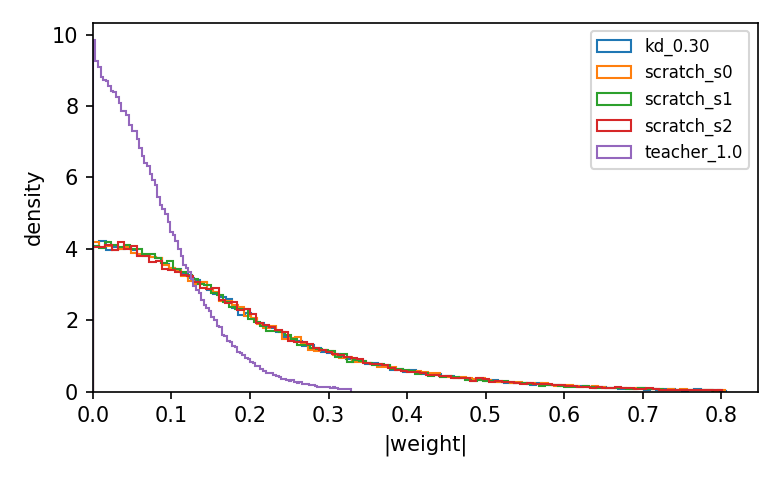
\includegraphics[width=\columnwidth]{figs/fig_weight_audit.png}
		\caption{Weight-magnitude audit: absolute convolutional and linear weights for the KD student, three fresh from-scratch seeds, and the teacher. Student and seeds overlap closely (the KD curve lies beneath the seed curves) with no heavy tails; the teacher's weights (a 6.3$\times$ larger pretrained model) are smaller and concentrate near zero.}
		\label{fig:weightaudit}
	\end{figure}
	
	\subsection{On-Device Latency over USB-Serial-JTAG}
	\label{sec:latency}
	
	\begin{figure}[h]
		\centering
		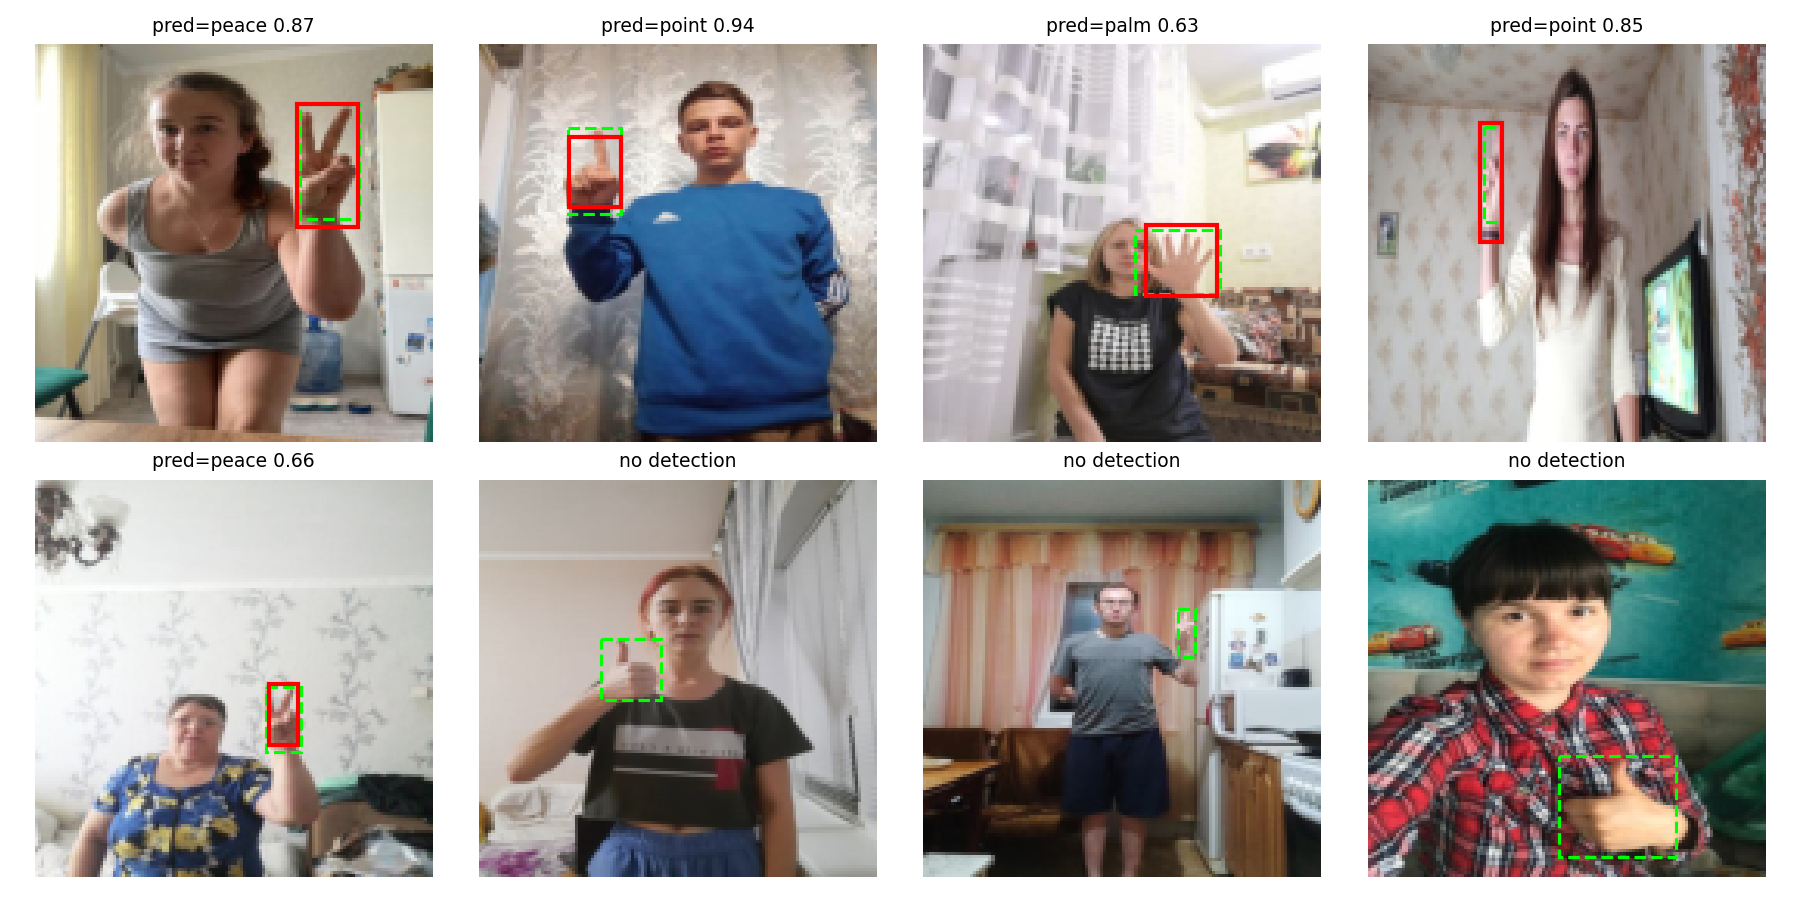
\includegraphics[width=\columnwidth]{figs/fig_demo_predictions.png}
		\caption{Example detection outputs for the distillation student (KD student, fp32, host-side) on the first 8 validation images (dashed green: ground truth; solid red: prediction).}
		\label{fig:demopred}
	\end{figure}
	
	\begin{table}[h]
		\caption{ESP32-S3 on-device latency, native USB-Serial-JTAG, $n=30$ repeated inferences per
			row (mean $\pm$ standard deviation), single fixed test image.}
		\label{tab:latency}
		\centering
		\resizebox{\columnwidth}{!}{%
			\begin{tabular}{llrrr}
				\toprule
				Model & Quant. & Infer.\ (ms) & Round trip (ms) & Overhead (\%) \\
				\midrule
				Scratch (0.3, seed-0)    & PTQ & $94.05 \pm 0.24$  & $190.51 \pm 0.67$ & $50.63 \pm 0.15$ \\
				Scratch (0.3, seed-0)    & QAT & $94.05 \pm 0.24$  & $191.32 \pm 1.05$ & $50.84 \pm 0.26$ \\
				KD student (0.3) & PTQ & $94.11 \pm 0.22$  & $191.32 \pm 0.92$ & $50.81 \pm 0.26$ \\
				KD student (0.3) & QAT & $94.10 \pm 0.22$  & $190.95 \pm 0.63$ & $50.72 \pm 0.19$ \\
				Pretrained (1.0) & PTQ & $468.35 \pm 0.38$ & $564.88 \pm 0.73$ & $17.09 \pm 0.09$ \\
				Pretrained (1.0) & QAT & $468.90 \pm 0.37$ & $565.95 \pm 1.10$ & $17.15 \pm 0.15$ \\
				\bottomrule
			\end{tabular}%
		}
	\end{table}
	
	Table~\ref{tab:latency} reports on-device inference and round-trip latency measured over the
	ESP32-S3's native USB-Serial-JTAG interface for all three training regimes, each in both its
	PTQ and QAT variant. Two findings stand out. First, on-device inference latency scales with
	model size (two widths tested), not quantization scheme: all four width-0.3 models (scratch and KD student
	alike, PTQ or QAT) infer in $\approx$94~ms, while both width-1.0 pretrained variants take
	$\approx$469~ms regardless of how they were quantized. This is the expected result, since PTQ
	and QAT produce the same INT8 execution graph structure at inference time and differ only in
	how the integer weights were obtained; the chip executes an identical sequence of operations
	either way, so the $\approx$5$\times$ latency gap between width 0.3 and width 1.0 is
	attributable entirely to backbone capacity, in line with MCU latency tracking operation count~\cite{banbury2021micronets}. Standard deviations are 0.2--0.4~ms on inference and 0.6--1.1~ms on round trip, so the differences among the four width-0.3 rows (at most 0.8~ms in round trip) lie within measurement spread.
	
	Second, the
	\emph{fixed} per-inference transfer and protocol overhead (image upload plus device receive
	time plus response parsing, consistently $\approx$96--97~ms in absolute terms across every
	row of Table~\ref{tab:latency}) consumes a different \emph{share} of total
	round-trip latency depending on model size: 50.6--50.8\% at width 0.3 against
	17.1--17.2\% at width 1.0. A fixed transport cost that does not shrink with the model takes a larger fraction of the smaller
	model's speed advantage. Optimizing model size without addressing the transfer path therefore
	leaves an increasing share of the achievable latency reduction unrealized as the model shrinks.
	For the width-0.3-class model that this paper favors on accuracy-per-parameter and
	accuracy-per-KB grounds (Sections~\ref{sec:width} and~\ref{sec:kd}), transfer overhead contributes about as much
	to total latency as inference itself and deserves matching engineering attention. These measurements were taken over USB-Serial-JTAG only, using a
	single repeatedly-inferred test image; they characterize timing and repeatability rather than
	on-device accuracy over the validation set, which Sections~\ref{sec:width} through~\ref{sec:ptqqat} establish separately
	from the full validation split, using the host-side INT8 reference executor.
	
	\section{Limitations and Scope}
	\label{sec:limits}
	
	The conclusions below come from one task, one toolchain, and a small number of runs, and six limits bound them.
	
	\emph{Statistics.} Most configurations are a single training run with seed 0 (the width-0.3 scratch, augmented and unaugmented, and KD families, three seeds each, are the exception), scored on one 433-image validation split that also drives checkpoint selection, calibration, and QAT epoch selection. Differences of about one F1 point, such as the 0.58-point gap between the QAT student and its fp32 counterpart or the 0.7-point spread across calibration sizes, cannot be separated from run-to-run noise with the present data. The large effects (pretraining plus augmentation, and distillation) lie far outside that range.
	
	\emph{QAT budget.} QAT uses a fixed 10-epoch budget at every capacity, which leaves the capacity explanation for the recovery ratio untested.
	
	\emph{Data.} The dataset is small (3{,}906 training and 433 validation images), pseudo-labeled with MediaPipe, and covers six visually distinct single-hand gestures. Magnitudes such as the 42\% distillation recovery describe this setting and may not carry over to cluttered, multi-object detection.
	
	\emph{Measurement and toolchain.} Latency was measured over USB-Serial-JTAG on a single test image, and all comparisons stay inside ESP-DL, with no TensorFlow Lite Micro baseline. Findings about the QAT workflow and about transfer overhead are therefore specific to this toolchain and interface.
	
	\emph{Width sweep.} The sweep is a single-seed, no-augmentation shape reference only (its width-0.3 run memorized the training images), and no-KD width-0.3 QAT figures are not reported.
	
	\emph{Unseparated effects and host-only accuracy.} At width 1.0, pretraining adds 8.3 F1 points over an augmented from-scratch model (single seeds). INT8 accuracy comes from the host reference executor, and no on-device accuracy run over the validation set was done.
	
	\section{Conclusion}
	
	This case study evaluated four interacting design levers (backbone width, ImageNet
	pretraining, knowledge distillation, and PTQ versus QAT) within a single, concrete ESP-DL
	deployment pipeline, with latency measured on real ESP32-S3 hardware and accuracy scored by the host-side INT8 reference executor, rather than in isolation. Four
	findings translate into concrete guidance for an engineer facing the same deployment problem.
	First, width selection should be driven by accuracy-per-parameter under the specific hardware
	budget at hand. The sweep is single-seed without augmentation; the 0.3 operating point is retained as the widest inside budget with a fresh three-seed baseline (59.70 $\pm$ 1.15 F1). Second, a pretrained, augmented teacher is worth training even when it cannot be deployed directly: it leads an augmented randomly initialized model by 8.3 F1 points at width 1.0, and the teacher's advantage over an augmented scratch student (27.2 F1 points) is partly recoverable at deployment budget through distillation: the distilled student closed about 42\% of that gap (11.3 points) while remaining under 90{,}000 parameters. Third, QAT recovered about half of the PTQ loss on the width-1.0 model in 10 epochs ($\approx$17\% of its 60-epoch schedule); no-KD width-0.3 QAT recovery is not reported, so QAT should be verified per deployment rather than assumed. Fourth, and most actionable for anyone deploying
	over a similar host-driven serial harness, per-inference transfer overhead does not shrink with the
	model, and a system optimized purely for small model size without corresponding attention to
	the transfer path will under-realize its own latency budget, particularly at the smaller end
	of the capacity range this style of deployment usually targets. These findings come from one six-class task, one toolchain, and mostly single-seed runs; Section~\ref{sec:limits} lists the limits on how far they generalize. Future work takes this pipeline to a 10-class COCO minitrain subset to test whether the pretraining, distillation, and quantization findings carry beyond single-hand gestures, alongside a fresh multi-seed width sweep.
	
	\section*{Acknowledgment}
	
	The authors thank the maintainers of ESP-DL and ESP-PPQ for tooling documentation, and the
	HaGRID and MediaPipe projects for dataset and annotation infrastructure used in this study.
	
	\begin{thebibliography}{00}
		
		\bibitem{esp32s3ds}
		Espressif Systems, ``ESP32-S3-WROOM-1 and ESP32-S3-WROOM-1U datasheet,'' v1.4. [Online]. Available: https://www.espressif.com/sites/default/files/documentation/esp32-s3-wroom-1\_wroom-1u\_datasheet\_en.pdf.
		
		\bibitem{david2021tflm}
		R.~David, J.~Duke, A.~Jain, V.~Janapa Reddi, N.~Jeffries, J.~Li, N.~Kreeger, I.~Nappier,
		M.~Natraj, T.~Wang, P.~Warden, and R.~Rhodes, ``TensorFlow Lite Micro: Embedded machine
		learning for TinyML systems,'' in \emph{Proc. Machine Learning and Systems (MLSys)}, vol.~3,
		2021, pp.~800--811.
		
		\bibitem{lin2020mcunet}
		J.~Lin, W.-M.~Chen, Y.~Lin, J.~Cohn, C.~Gan, and S.~Han, ``MCUNet: Tiny deep learning on IoT
		devices,'' in \emph{Advances in Neural Information Processing Systems (NeurIPS)}, vol.~33,
		2020, pp.~11711--11722.
		
		\bibitem{jacob2018quantization}
		B.~Jacob, S.~Kligys, B.~Chen, M.~Zhu, M.~Tang, A.~Howard, H.~Adam, and D.~Kalenichenko,
		``Quantization and training of neural networks for efficient integer-arithmetic-only
		inference,'' in \emph{Proc. IEEE Conf. Computer Vision and Pattern Recognition (CVPR)}, 2018,
		pp.~2704--2713.
		
		\bibitem{espdlguide}
		Espressif Systems, ``ESP-DL,'' GitHub repository. [Online]. Available: https://github.com/espressif/esp-dl.
		
		\bibitem{sandler2018mobilenetv2}
		M.~Sandler, A.~Howard, M.~Zhu, A.~Zhmoginov, and L.-C.~Chen, ``MobileNetV2: Inverted residuals
		and linear bottlenecks,'' in \emph{Proc. IEEE Conf. Computer Vision and Pattern Recognition
			(CVPR)}, 2018, pp.~4510--4520.
		
		\bibitem{liu2016ssd}
		W.~Liu, D.~Anguelov, D.~Erhan, C.~Szegedy, S.~Reed, C.-Y.~Fu, and A.~C.~Berg, ``SSD: Single
		shot multibox detector,'' in \emph{Proc. European Conf. Computer Vision (ECCV)}, 2016,
		pp.~21--37.
		
		\bibitem{kapitanov2024hagrid}
		A.~Kapitanov, K.~Kvanchiani, A.~Nagaev, R.~Kraynov, and A.~Makhliarchuk, ``HaGRID -- HAnd
		Gesture Recognition Image Dataset,'' in \emph{Proc. IEEE/CVF Winter Conf. Applications of
			Computer Vision (WACV)}, 2024, pp.~4572--4581.
		
		\bibitem{lai2018cmsisnn}
		L.~Lai, N.~Suda, and V.~Chandra, ``CMSIS-NN: Efficient neural network kernels for Arm
		Cortex-M CPUs,'' \emph{arXiv preprint arXiv:1801.06601}, 2018.
		
		\bibitem{banbury2021mlperftiny}
		C.~Banbury \emph{et al.}, ``MLPerf Tiny benchmark,'' in \emph{Advances in Neural Information Processing Systems (NeurIPS), Datasets and Benchmarks Track}, 2021, arXiv:2106.07597.
		
		\bibitem{espdldocs}
		Espressif Systems, ``How to quantize model,'' \emph{ESP-DL User Guide}. [Online]. Available: https://docs.espressif.com/projects/esp-dl/en/latest/tutorials/how\_to\_quantize\_model.html.
		
		\bibitem{nagel2021whitepaper}
		M.~Nagel \emph{et al.}, ``A white paper on neural network quantization,'' \emph{arXiv preprint arXiv:2106.08295}, 2021.
		
		\bibitem{hinton2015distilling}
		G.~Hinton, O.~Vinyals, and J.~Dean, ``Distilling the knowledge in a neural network,''
		\emph{arXiv preprint arXiv:1503.02531}, 2015.
		
		\bibitem{chen2025animalreid}
		Y.~Chen, D.~Zhao, Y.~S.~Koh, and T.~Xu, ``Animal re-identification on microcontrollers,'' \emph{arXiv preprint arXiv:2512.08198}, 2025.
		
		\bibitem{karjol2026edgekd}
		A.~Karjol and D.~M.~Hanna, ``Edge AI for automotive vulnerable road user safety: Deployable
		detection via knowledge distillation,'' \emph{arXiv preprint arXiv:2604.26857}, 2026.
		
		\bibitem{zhang2020mediapipe}
		F.~Zhang \emph{et al.}, ``MediaPipe Hands: On-device real-time hand tracking,'' \emph{arXiv preprint arXiv:2006.10214}, 2020.
		
		\bibitem{he2019rethinking}
		K.~He, R.~Girshick, and P.~Doll\'ar, ``Rethinking ImageNet pre-training,'' in \emph{Proc. IEEE/CVF Int. Conf. Computer Vision (ICCV)}, 2019, pp.~4918--4927.
		
		\bibitem{banbury2021micronets}
		C.~Banbury \emph{et al.}, ``MicroNets: Neural network architectures for deploying TinyML applications on commodity microcontrollers,'' \emph{arXiv preprint arXiv:2010.11267}, 2020.
		
	\end{thebibliography}
	
\end{document}